\section{Quantum Modular\\ Multiplication}
\label{sec:csa-mod-mult}

We can build upon our carry-save adder to implement quantum modular
multiplication in logarithmic depth. We start with a completely classical
problem to illustrate the principle of multiplication by repeated addition.
Then we consider modular multiplication of two quantum numbers in a serial
and a parallel fashion in
\ref{subsec:csa-mod-mult-qq}. Both of these problems use as a subroutine the
generic problem of \emph{modular multiple addition} which we define and solve
in \ref{subsec:mma}.

%%%%%%%%%%%%%%%%%%%%%%%%%%%%%%%%%%%%%%%%%%%%%%%%%%%%%%%%%%%%%%%%%%%%%%%%%%%%%%%
First we consider a completely classical problem:
given three $n$-bit classical numbers $a$, $b$, and $m$,
compute $c = ab \bmod m$, where $c$ is allowed to be in CSE.

We only have to add shifted
multiples of $a$ to itself, ``controlled'' on the bits of $b$. There are
$n$ shifted multiples of $a$, let's call them $z^{(i)}$, one for every bit of $b$:
%%\begin{equation}
$z^{(i)} = 2^i a b_i \bmod m$.
%%\end{equation}
We can parallelize the addition of $n$ numbers in a logarithmic depth
binary tree to get a total depth of $O(\log n)$.

%%%%%%%%%%%%%%%%%%%%%%%%%%%%%%%%%%%%%%%%%%%%%%%%%%%%%%%%%%%%%%%%%%%%%%%%%%%%%%
\subsection{Modular Multiplication of\\ Two Quantum Numbers}
\label{subsec:csa-mod-mult-qq}

We now consider the problem of multiplying a classical number controlled
on a quantum bit and a
\emph{quantum number},\footnote{In this paper, quantum
numbers often result by entangling a classical number in one register with a
quantum control bit. This should not be confused with the physics meaning
of a quantum number.} which is a
quantum superposition of classical numbers:
%\begin{quote}
given an $n$-qubit quantum number $\ket{x}$, a control qubit $\ket{p}$,
and two $n$-bit classical numbers $a$
and $m$,
compute $\ket{c} = \ket{xa[m]}$, where $c$ is allowed to be in CSE.
This problem occurs naturally in modular exponentiation (described in
the next section) and can be considered \emph{serial multiplication},
in that $t$ quantum numbers are multiplied in series to a single
quantum register.
%\end{quote}

We first create $n$ quantum numbers $\ket{z^{(i)}}$,
which are shifted multiples of the classical number $a$ controlled on the bits
of $x$:
%\begin{equation}
$\ket{z^{(i)}} \equiv \ket{2^i a[m] \cdot x_i }$.
%\end{equation}
How do we create these numbers, and what is the depth of the procedure?
First, note that $\ket{2^i a[m]}$ is a classical number, so we can
precompute this classically and prepare them in parallel using single-qubit
operations
on $n$ registers, each consisting of $n$ ancillae qubits. Each $n$-qubit
register will hold a future $\ket{z^{(i)}}$ value.
We then copy all
$n$ bits of $x$, $n$ times each, using an unbounded fanout operation so that
$n$ copies of each bit $\ket{x_i}$ is next to register $\ket{z^{(i)}}$.
This takes a total of $O(n^2)$ parallel CNOT operations.
We then entangle each $\ket{z^{(i)}}$ with the corresponding $x_i$.
The schematic for this is shown in Figure \ref{fig:mod-mult-create}, not
showing how we interleave these numbers into groups of three using
constant-depth teleportation. This reduces to the task of modular
multiple addition, in order to add these numbers down to a single
number modulo $m$, which is described in \ref{subsec:mma}.

\begin{figure*}[htp!]
\centerline{
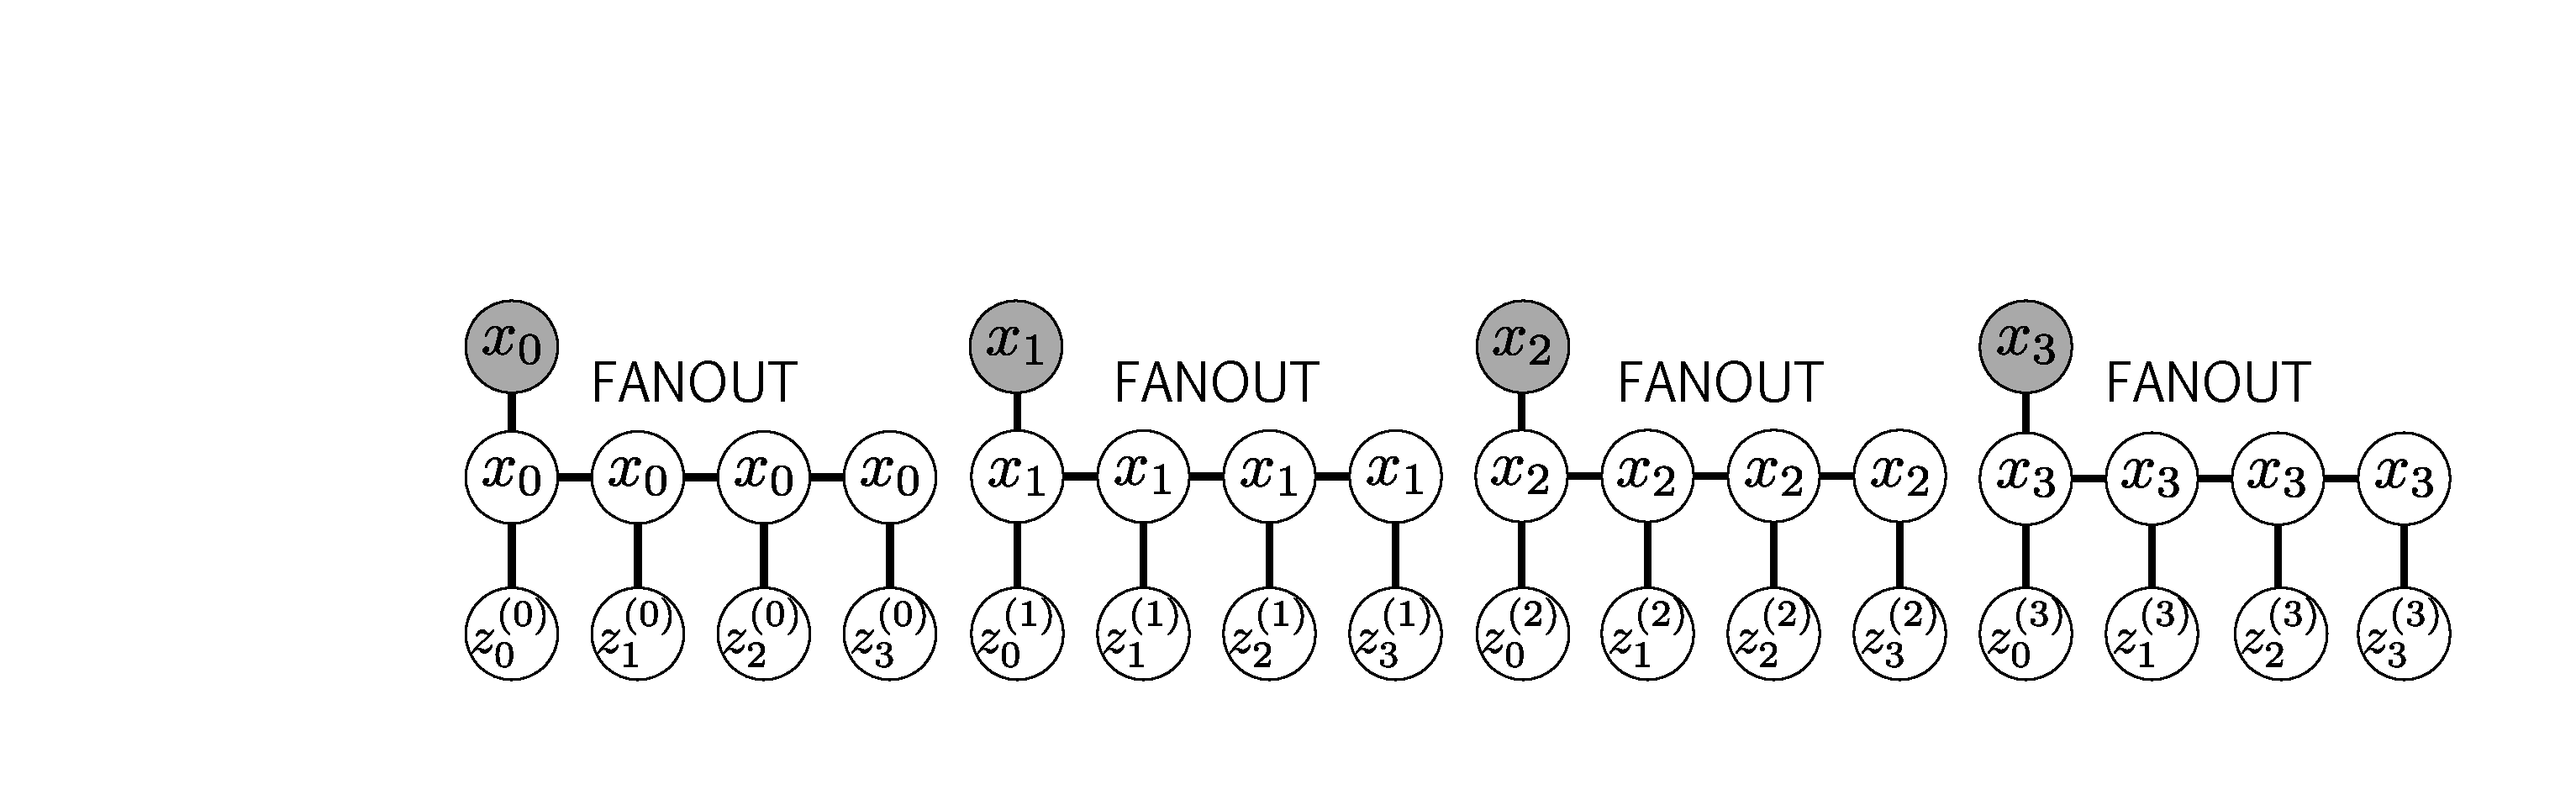
\includegraphics[width=4.5in]{figures/znumbers.pdf}
}
\caption{Creating $n=4$ shifted values $\{z^{(0)},z^{(1)},z^{(2)},z^{(3)}\}$
for an input number $x$.}
\label{fig:mod-mult-create}
\end{figure*}

Finally, we tackle the most interesting problem:
%\begin{quote}
given two $n$-qubit quantum numbers $\ket{x}$ and
$\ket{y}$ and a $n$-bit classical number
$m$,
compute $\ket{c} = \ket{xy \bmod m}$,
where $\ket{c}$ is allowed to be in CSE.
This can be considered \emph{parallel multiplication} and is responsible
for our logarithmic speedup in modular exponentiation.
%\end{quote}

Instead of creating $n$ quantum numbers $\ket{z^{(i)}}$, we must create
$n^2$ numbers
$\ket{z^{i,j}}$ for all possible pairs of quantum bits $x_i$ and $y_j$,
$i,j \in \{0,\ldots,n-1\}$:
%\begin{equation}
$\ket{z^{i,j}} \equiv \ket{2^i2^j[m]\cdot x_i \cdot y_j}$.
%\end{equation}
We create these numbers using a similar procedure to the previous problem.
Adding $n^2$ quantum numbers of $n$ qubits each takes depth
$O(\log(n^2))$ which is still $O(\log n)$.
Creating $n^2\times n$-bit quantum numbers takes width $O(n^3)$. 

%%%%%%%%%%%%%%%%%%%%%%%%%%%%%%%%%%%%%%%%%%%%%%%%%%%%%%%%%%%%%%%%%%%%%%%%%%%%%%%
\subsection{Modular Multiple Addition}
\label{subsec:mma}

As a subroutine to modular multiplication, we define the operation of
repeatedly adding multiple numbers down to a single CSE number, called
\emph{modular multiple addition}.

The modular multiple addition circuit generically adds down $t\times n$-bit
conventional numbers to an $n$-bit CSE number.
%
\begin{equation}
z^{(0)} + z^{(1)} + \ldots z^{(n-1)} \equiv (u+v)[m]
\end{equation}
%
It does not matter how the
$t$ numbers are generated, as long as they are divided into groups of three
and have their bits interleaved to be the inputs of a CSA tile.
In the cases above, serial multiplication results in
$t = n$ and parallel multiplication results in $t = n^2$.
At the beginning of the circuit, all CSA tiles are
\emph{active} in that they have tile input numbers $z^{(i)}$
to multiply, and their tile outputs will affect the overall circuit output,
$u+v$.

As the circuit proceeds through a number of timesteps,
tiles will become \emph{inactive} when they
do not receive new numbers for their tile inputs; at
that point, their tile outputs can no longer affect the circuit output.
Since the CSA tile is a 3-2 adder, one can see that if there are $t$ CSA tiles
active at the beginning of a timestep, there are $\lceil 2t/3 \rceil$ active
tiles at the end of the timestep, since there are roughly two-thirds as many
input numbers left to add down to the circuit output $u+v$. One can see that
the total number of timesteps
is therefore $\lceil \log_{3/2}(t/3) \rceil + 1$.

To facilitate the below discussion, we will assign colors to each CSA tile,
which are updated during the circuit execution. Active tiles can either be
black or gray.
A \emph{black} tile will keep its two output numbers as inputs and receive
a third input number. An exception is the rightmost black tile may teleport
one of its output numbers to its left black nearest neighbor and receive
two input numbers from its right gray nearest neighbor.
A \emph{gray} tile will teleport one of its output
numbers to the nearest active tile to its left and the other output number
to the nearest active tile to its right. An exception is the rightmost gray
tile may teleport both output numbers to its left black nearest neighbor.
We can think of inactive tiles as
\emph{white} tiles in that they ``fade'' out of the circuit, and numbers
get teleported through them without stopping to be added. The symbols for
these colors are shown in Figure \ref{fig:tile-colors}.

\begin{figure*}[htb!]
\centerline{
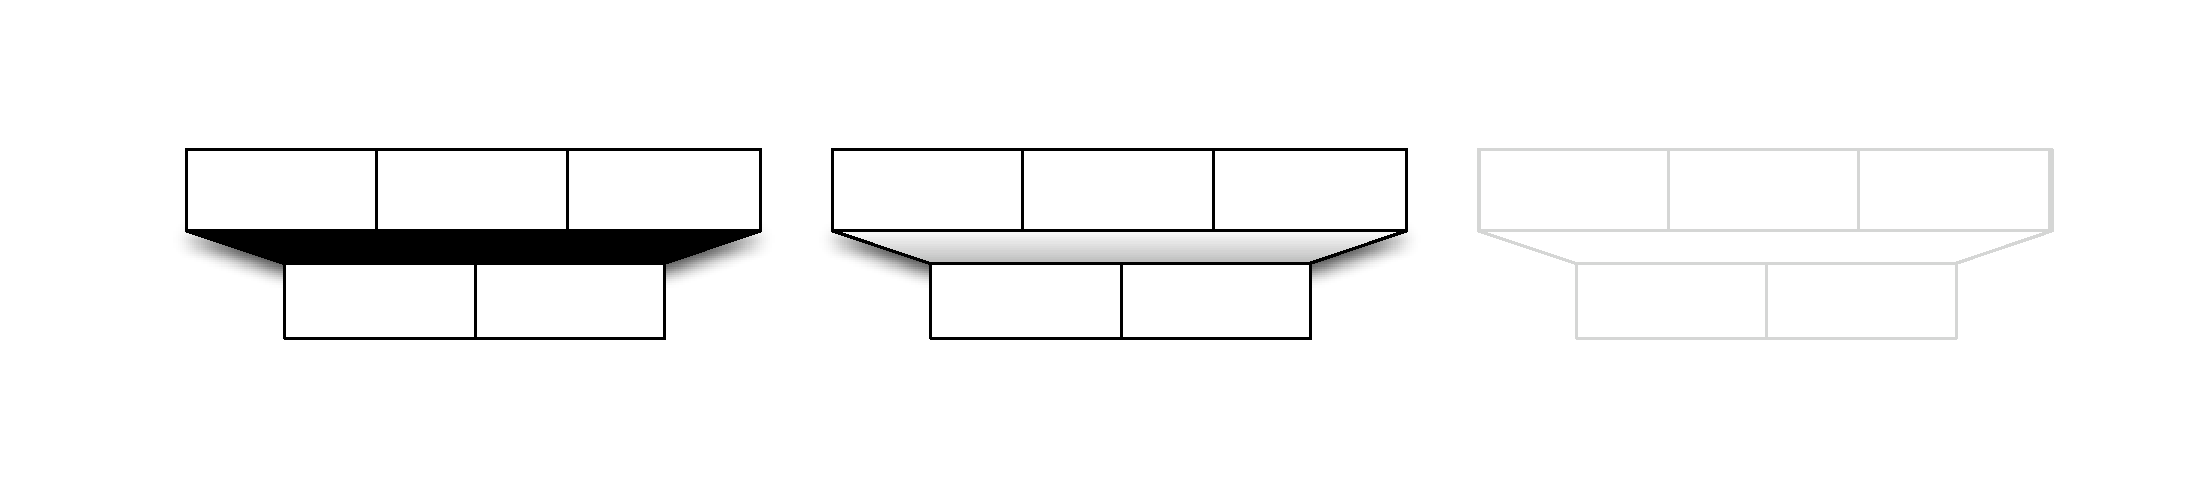
\includegraphics[width=5.5in]{figures/csa-tile-colors.pdf}
}
\caption{From left to right, the symbols for a black, gray, and white tile,
respectively.}
\label{fig:tile-colors}
\end{figure*}


The rules for
updating tiles at the end of each timestep are as follows:

\begin{itemize}
\item \textbf{Black tiles} are always active for the next timestep, but
change colors as follows.
\begin{itemize}
\item The leftmost tile always stays black.
\item If a black tile has a gray tile as its nearest active right neighbor in
the current timestep,
it stays \textbf{black} in the next timestep.
\item If a black tile has a black tile as its nearest active neighbor either
to the right or the left, and it is not the leftmost tile,
it turns \textbf{gray} in the next timestep.
\end{itemize}
\item \textbf{Gray tiles} always turn white (inactive) in the next timestep.
\end{itemize}

The initial state of the tile colors depends on its index
$i \in \{0, 1, \ldots, q-1\}$ within $q = \lceil t/3 \rceil$ tiles.

\begin{itemize}
\item If $i \bmod 3 = 0$, then it starts out black.
\item If $i \bmod 3 = 1$, then it starts out gray.
\item If $i \bmod 3 = 2$, then it starts out black.
\end{itemize}

Given the rules above, one can see that the leftmost tile stays black
throughout the entire circuit, and holds the final output number $(u+v)$ at
the end.

Each timestep of the circuit consists of the following operations:

\begin{enumerate}
\item
All active CSA tiles will execute in
parallel to transform their three input numbers into two output numbers
(a CSE number).
\item
Gray tiles teleport their output numbers to the left and to the right to
their black tile neighbors. The exception is the rightmost gray tile will
teleport both of its output numbers to its left black tile nearest neighbor.
\item
Tile colors will change according to the rules above. Approximately
two-thirds of the tiles will
become inactive in the next timestep.
\item
Go back to Step 1 for the next timestep.
\end{enumerate}

These steps and the above tile color rules are best illustrated with a concrete
example. In Figure \ref{fig:mod-mult}, we see the circuit for modular
multiple addition as a series of
snapshots, separated by heavy dotted lines, with the passage of time going
downward. The tiles change color over time, and the arrows indicate the
teleportation of output numbers to neighboring active tiles in each timestep.
In the initial timestep, the tiles are numbered to show how they are assigned
their initial color.
Between Timestep 0 and Timestep 1,
all $\lceil n/3 \rceil$ CSA tiles are active. After each succeeding timestep,
$\lfloor 2/3 \rfloor$
fewer CSA tiles are active until the very end, when only one CSA tile is
active. By the convention established above,
we teleport the rightmost output numbers to the left, so that the
final output is read out from the leftmost CSA tile.

\begin{figure*}[htb!]
\centerline{
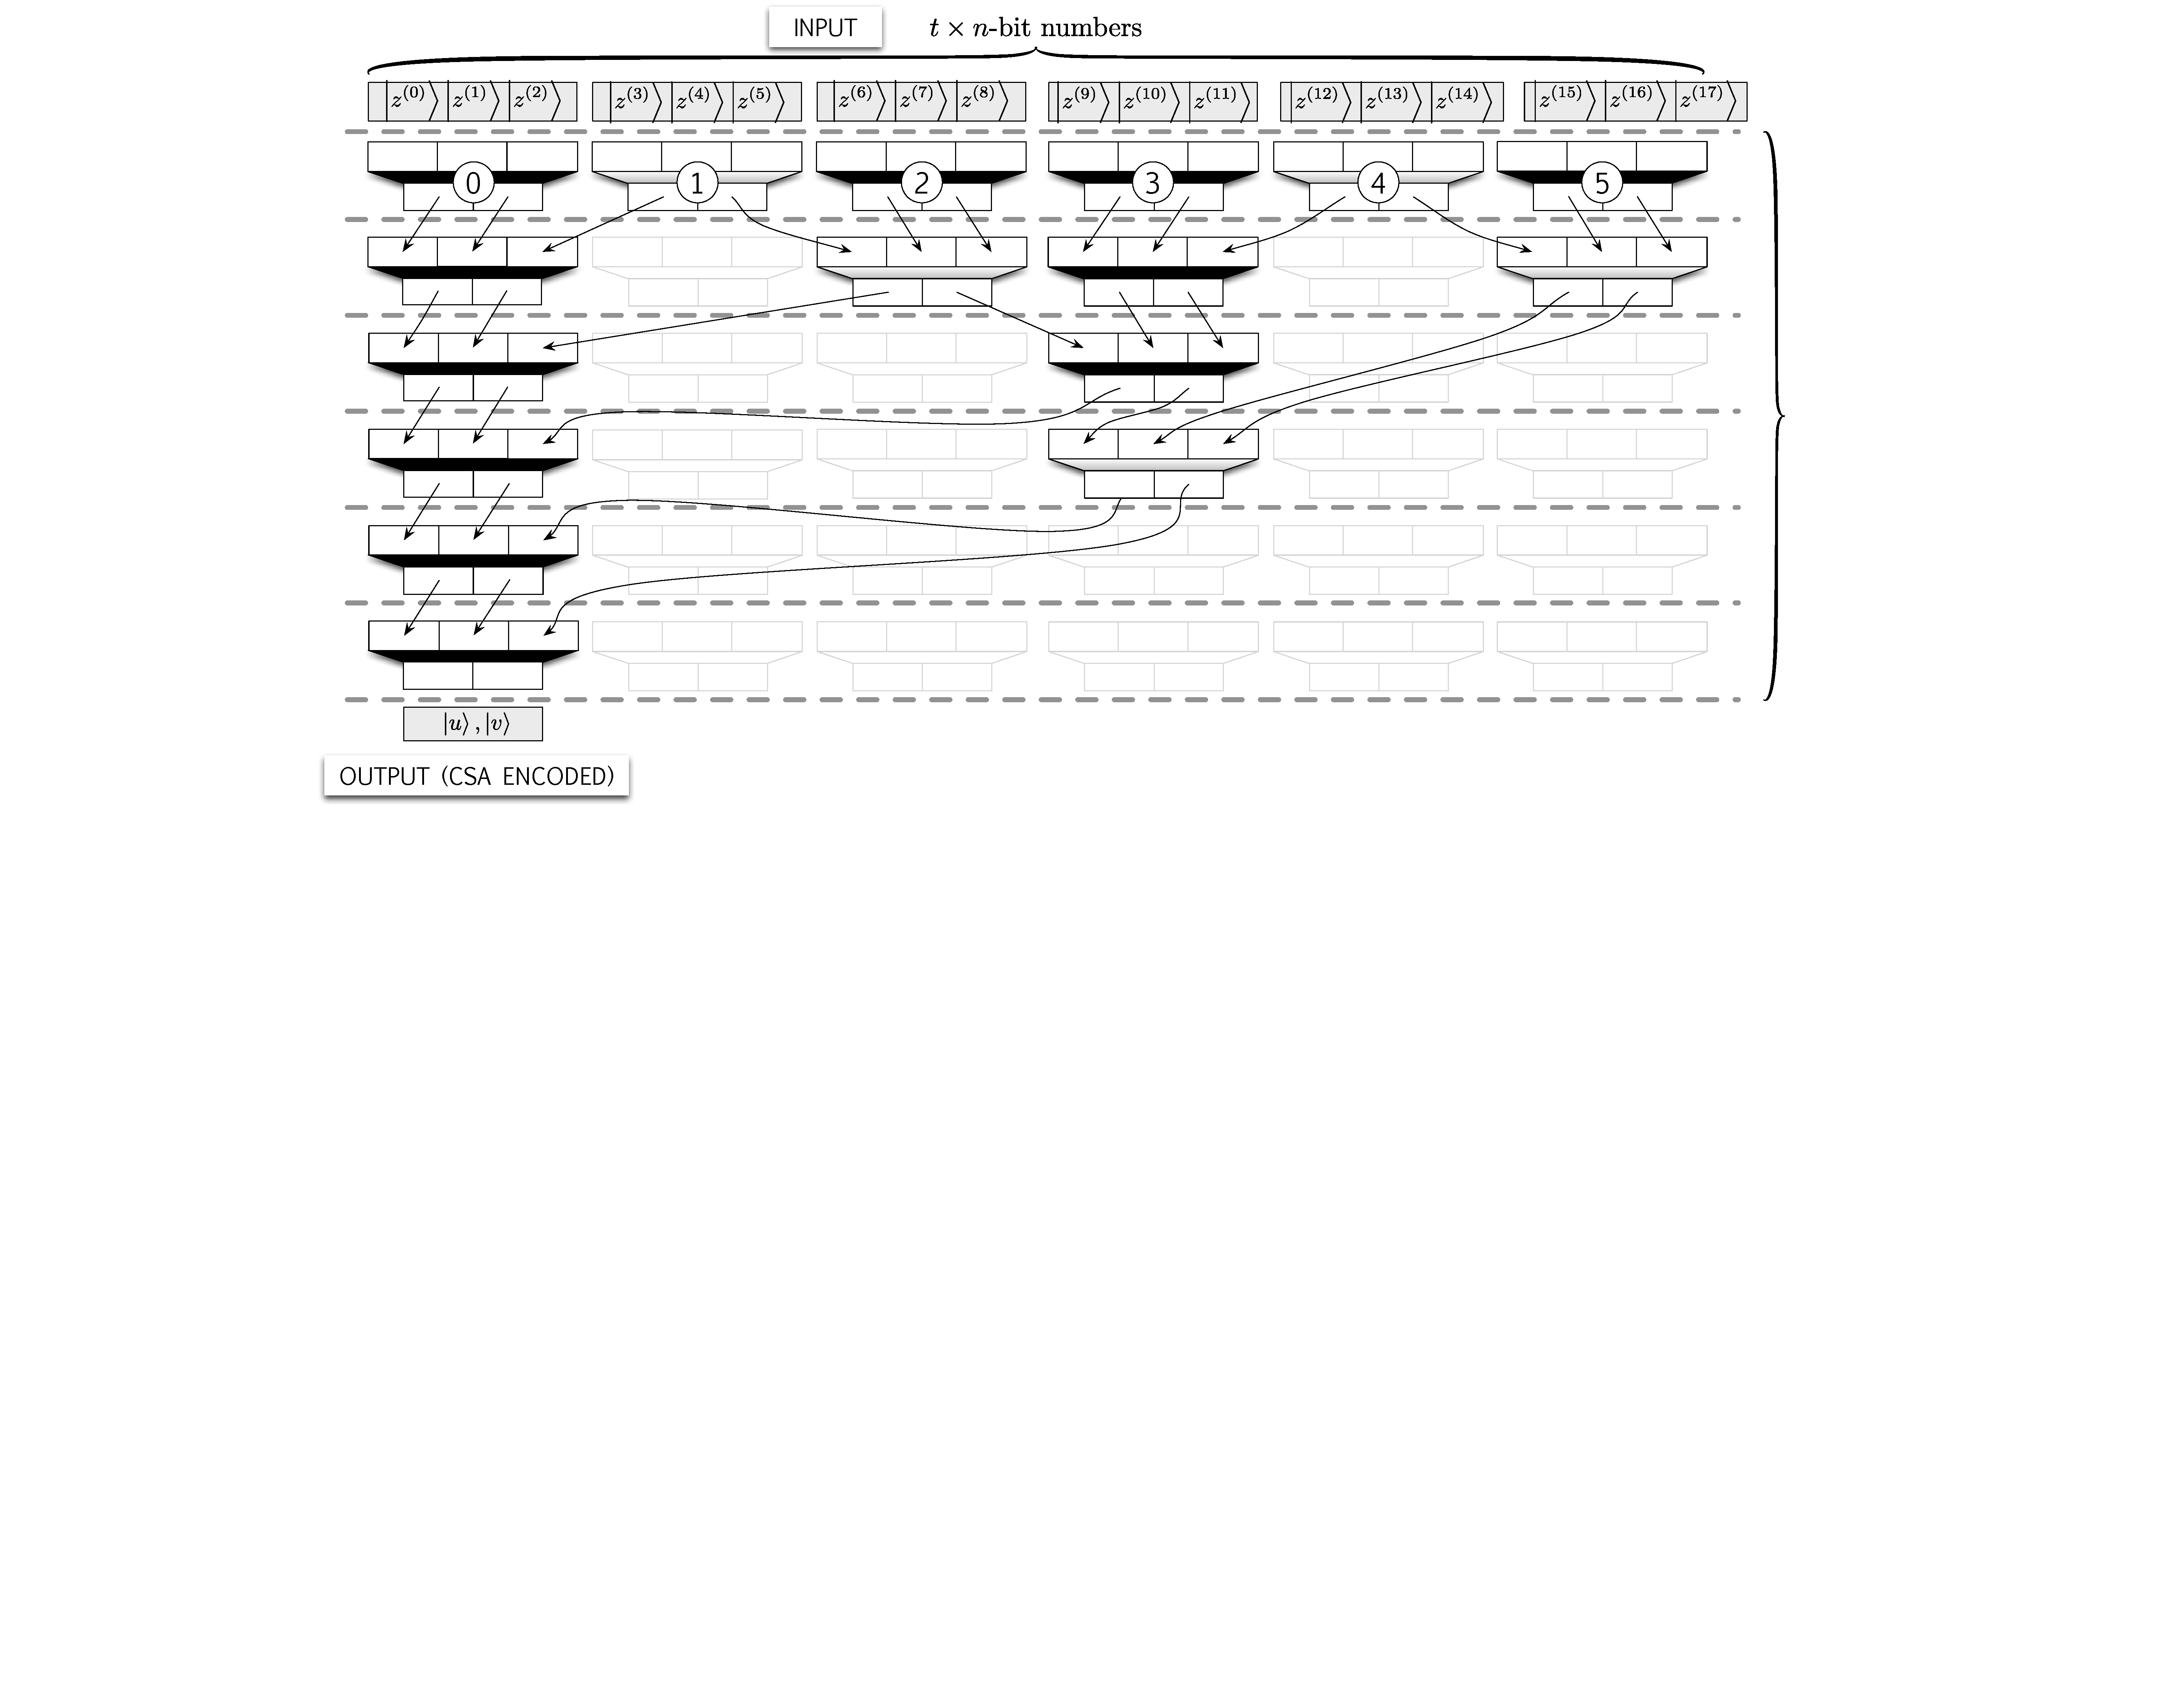
\includegraphics[width=6.5in]{figures/mod-mult-add.pdf}
}
\caption{Modular multiple addition of quantum numbers on a CSA tile
architecture for $t=18$ with depth $(\lceil \log_{\frac{3}{2}}(t/3) \rceil + 1) = 6$
timesteps}
\label{fig:mod-mult}
\end{figure*}
%

Now we can analyze the circuit resources for multiplying $n$-bit
quantum numbers, which requires $(t-2)$ modular additions, for $t=n^2$.
The circuit width is the sum of the $O(n^3)$ ancillae
needed for number generation and the ancillae required for $O(n^2)$
modular additions. Each modular addition has width $O(n)$ and depth $O(1)$
from the previous
section. There are
$\lceil \log_{3/2}(n^2 / 3) \rceil +1 $ timesteps of modular addition. Therefore
the entire modular multiplier circuit has depth $O(\log n)$ and width $O(n^3)$.
